% http://tex.stackexchange.com/questions/11866/compile-a-latex-document-into-a-png-image-thats-as-short-as-possible#11880
%http://tex.stackexchange.com/questions/152247/best-practice-to-include-standalone-precompiled-graphics
\documentclass[border=1pt]{standalone}
\usepackage{tikz}

\begin{document}

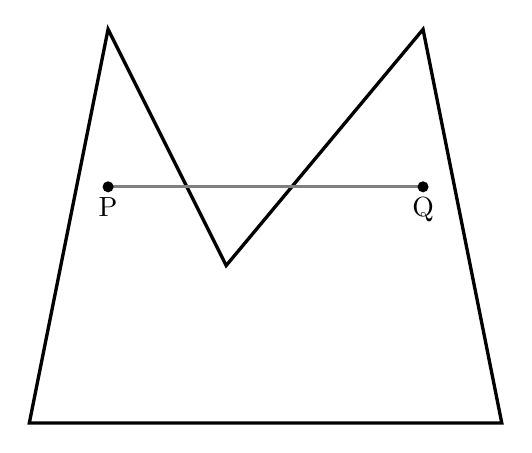
\begin{tikzpicture}[very thick]
	%\coordinate (A1) at (0,0);
	%\coordinate (A2) at (6, 4);
	%\draw [help lines, lightgray] (A1) grid (A2);

	% convex set
	\draw (0,0) -- (6,0) -- (5,5) -- (2.5,2) -- (1,5) -- cycle;
	\newcommand {\lsy}{3}
	\coordinate (P) at (1,\lsy); \coordinate (Q) at (5,\lsy);
	\draw[gray] (P) -- (Q);
	\node[below] at (P) {P};
	\node[below] at (Q) {Q};
	\fill (1,\lsy) circle [radius=2pt];
	\fill (5,\lsy) circle [radius=2pt];

\end{tikzpicture}

\end{document}
